\subsection*{20.1}
What is consumer surplus, producer surplus and total surplus in autarky and after trade?
\begin{figure}[H]
    \centering
    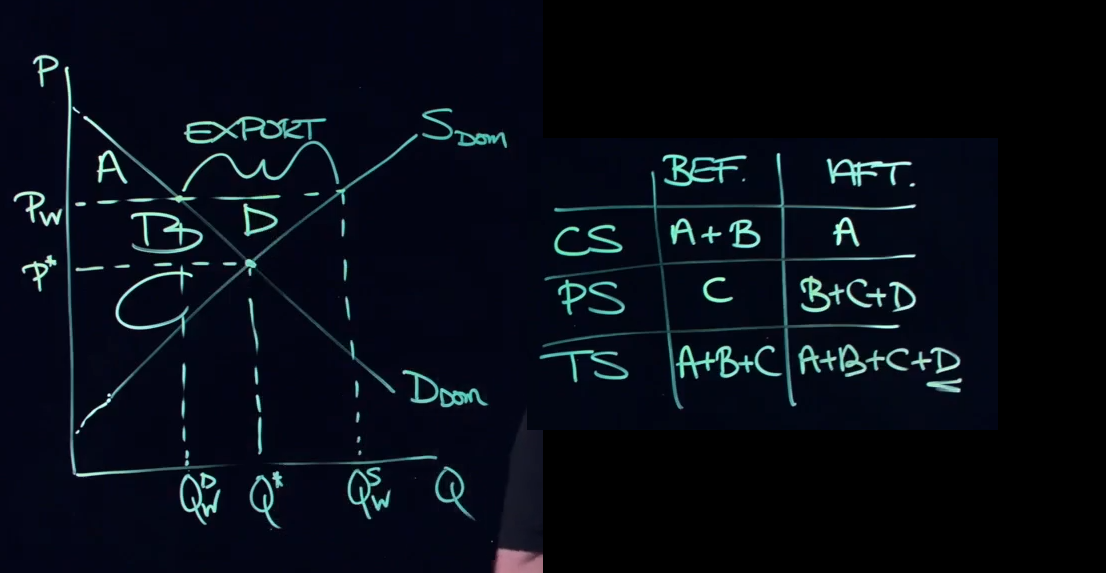
\includegraphics[width=0.5\textwidth]{Chapter20/ExportSurplus.png}
    \caption{Export Surplus}
    \label{fig:exportsurplus}
\end{figure}
\begin{figure}[H]
    \centering
    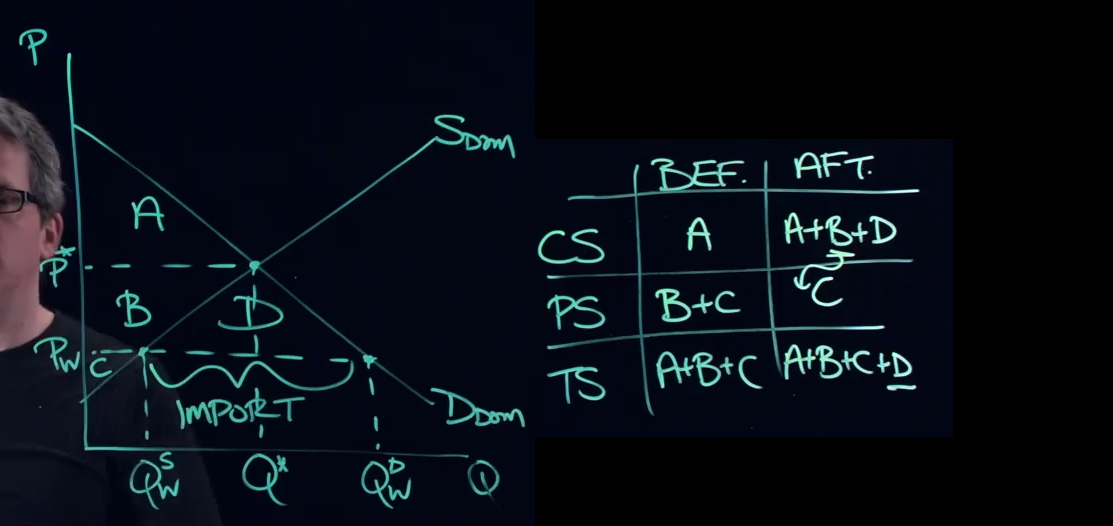
\includegraphics[width=0.5\textwidth]{Chapter20/ImportSurplus.png}
    \caption{Import Surplus}
    \label{fig:importsurplus}
\end{figure}
Going from free trade to autarky will always reduce total surplus.\\
Deepening trade ties makes the world a safer place.\\
There are valid (invalid) and invalid (even more invalid) arguments against free trade.
\begin{itemize}
    \item Valid: 
    \begin{itemize}
        \item Opposing trade allows for diversification.\\
        The counter-argument is why would you want to protect a market when another country can do it more efficiently.
        The industry should not be protected.
        \item We should try to protect certain industries because certain groups will like it.\\
        The counter-argument is that the gains from trade are greater than the losses.
        \item By blocking trade, you may improve the terms of trade.\\
        The counter-argument is that the gains from trade have nothing to do with the terms of trade.
        \item The infant industry argument: protect the industry until it can compete, 
        with enough time the country will be an exporter instead of an importer.\\
        The counter-argument is that it is very difficult to take away government protection once it is given.
        \item What if by blocking trade, we stand the ability to gain profits that we wouldn't be able to get. This is the issue of appropriability.\\
        It's foolish to think that if there are profits to be made, other countries won't be doing the same thing to get them.
    \end{itemize}
    \item Invalid:
    \begin{itemize}
        \item This will keep money at home.\\
        The counter-argument is that canadian money is not useful in other countries.
        \item We should protect ourselves against cheap labour.\\
        The counter-argument is that its an issue of productivity, not labour.
        \item Exports are a good thing but imports are not.\\
        This is known as mercantilism. The counter-argument is that you cannot have one without the other. Exports pay for imports.
        \item This protects domestic jobs.\\
        The counter-argument is that if a job needs protecting, you are not good at it.
    \end{itemize}
\end{itemize}